\begin{figure}
	\centering
	\subfigure[$\Delta t$ = 1 día]{
	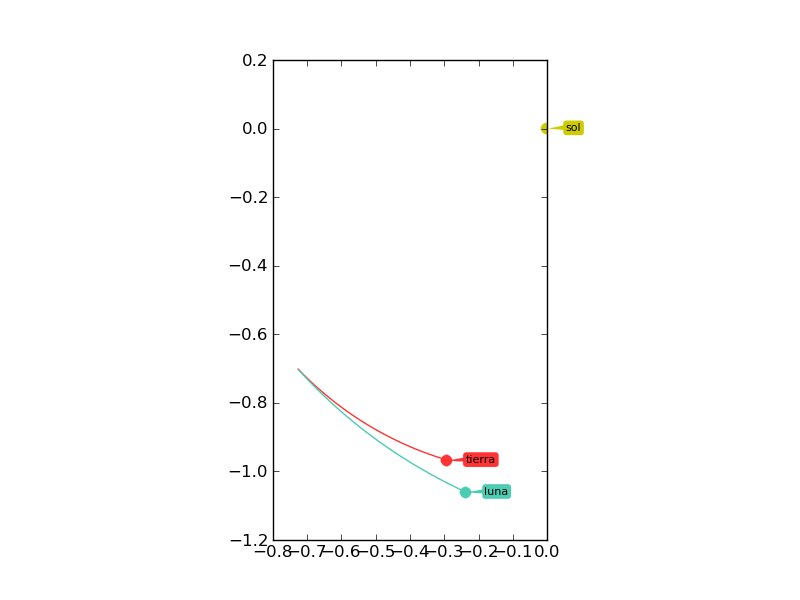
\includegraphics[scale=0.38]{img/ej1/metodo2/validacion_30_1.png}
	\label{fig:ej1_m2_30_1}
	}
	\subfigure[$\Delta t$ = 6 horas]{
	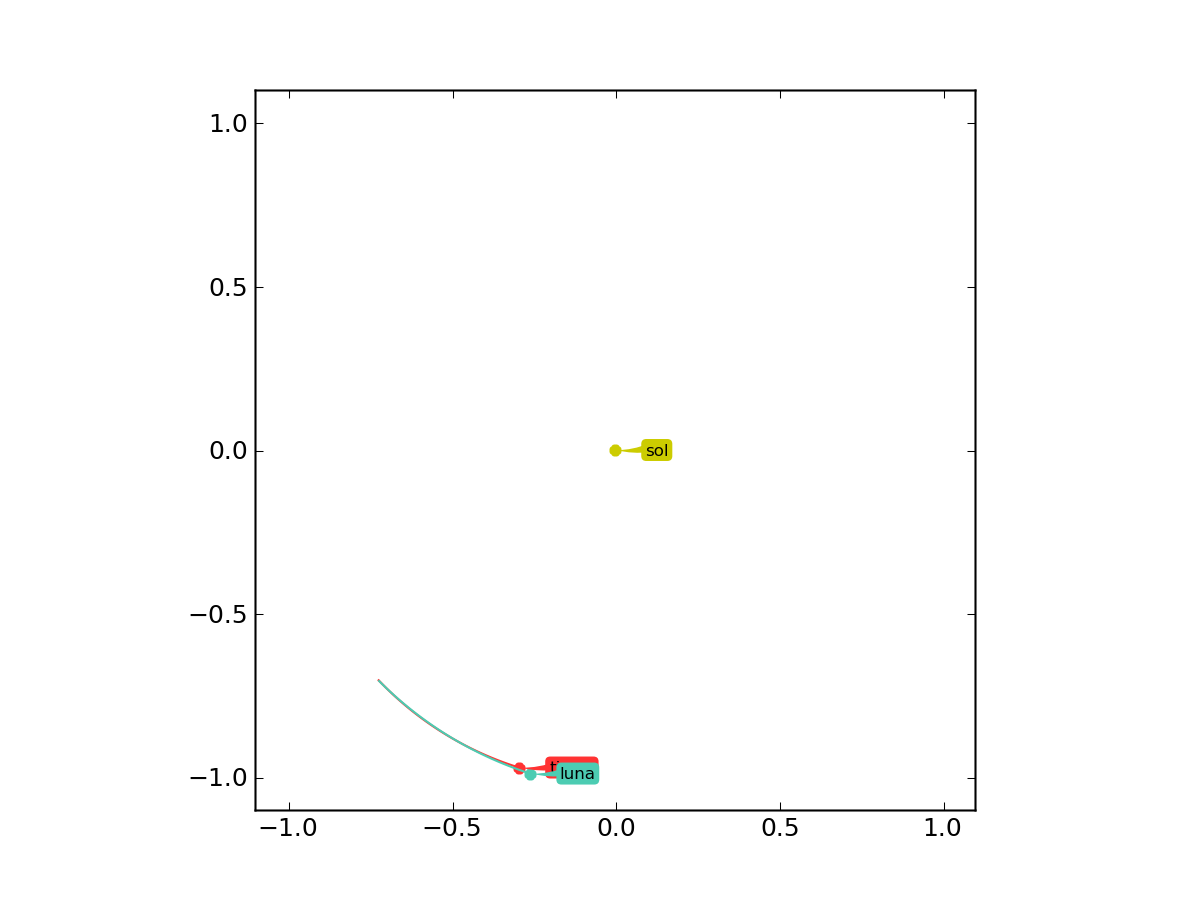
\includegraphics[scale=0.38]{img/ej1/metodo2/validacion_30_4.png}
	\label{fig:ej1_m2_30_4}
	}
	\\
	\subfigure[$\Delta t$ = 2 horas]{
	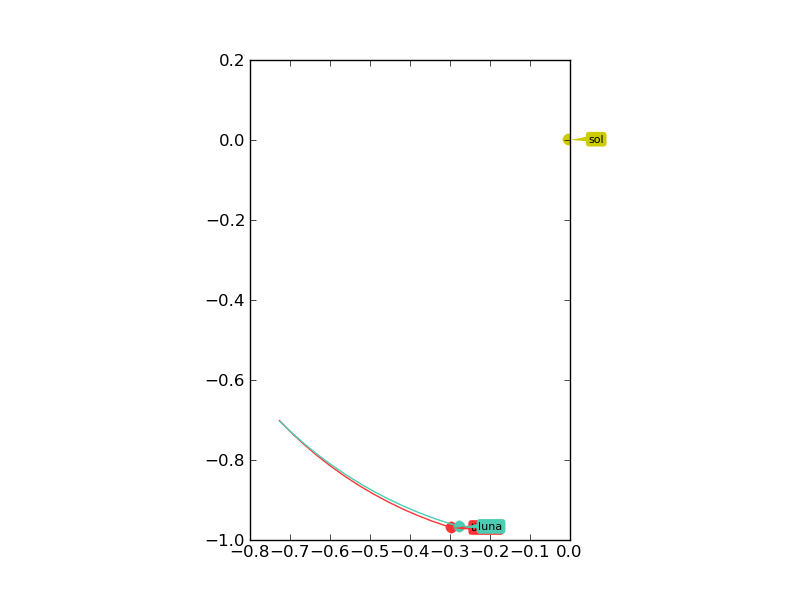
\includegraphics[scale=0.38]{img/ej1/metodo2/validacion_30_12.png}
	\label{fig:ej1_m2_30_12}
	}
	\subfigure[$\Delta t$ = 1 hora]{
	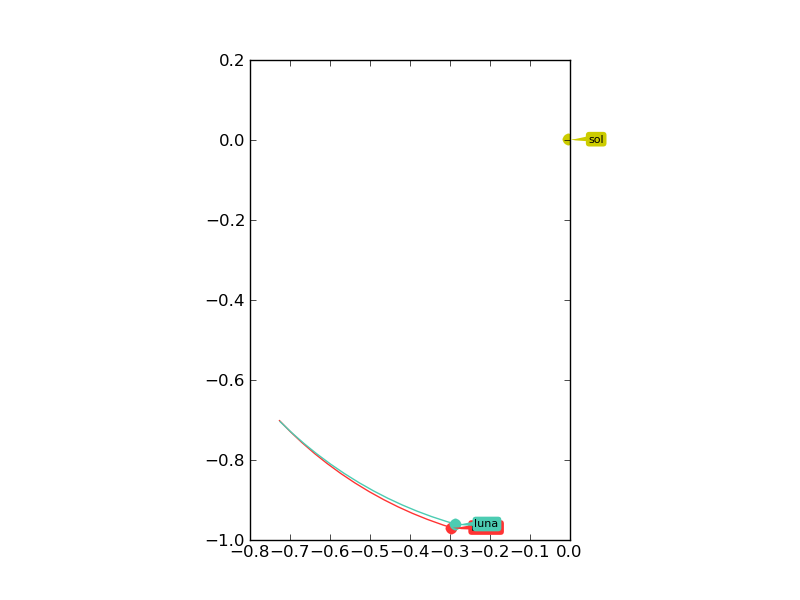
\includegraphics[scale=0.38]{img/ej1/metodo2/validacion_30_24.png}
	\label{fig:ej1_m2_30_24}
	}
	\caption{
		Simulación de validación del sistema sol$-$tierra$-$luna para un período de 30 días y distintos $\Delta t$
		con el método 2.
		Al parecer el método 2 tiende a ser mas sensible a los errores por discretizacion del tiempo que el 1,
		ya que para un intervalo de tiempo pequeño, como lo es 1 mes,
		notamos cambios importantes en la precision con un $\Delta t$ grande (1 día) con respecto al método 1.
	}
	\label{ fig:res_ej1_m2_30 }
\end{figure}
\begin{figure}
	\centering
	\subfigure[$\Delta t$ = 1 día]{
	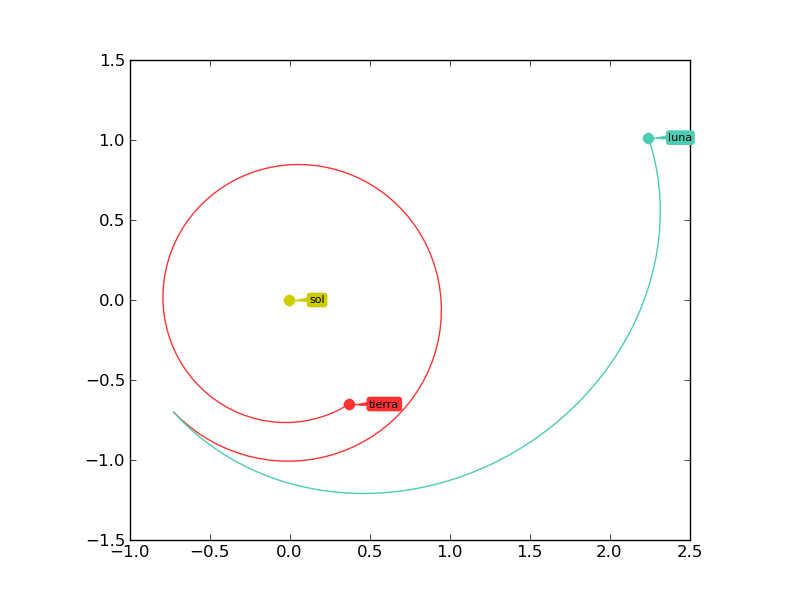
\includegraphics[scale=0.38]{img/ej1/metodo2/validacion_365_1.png}
	\label{fig:ej1_m2_365_1}
	}
	\subfigure[$\Delta t$ = 6 horas]{
	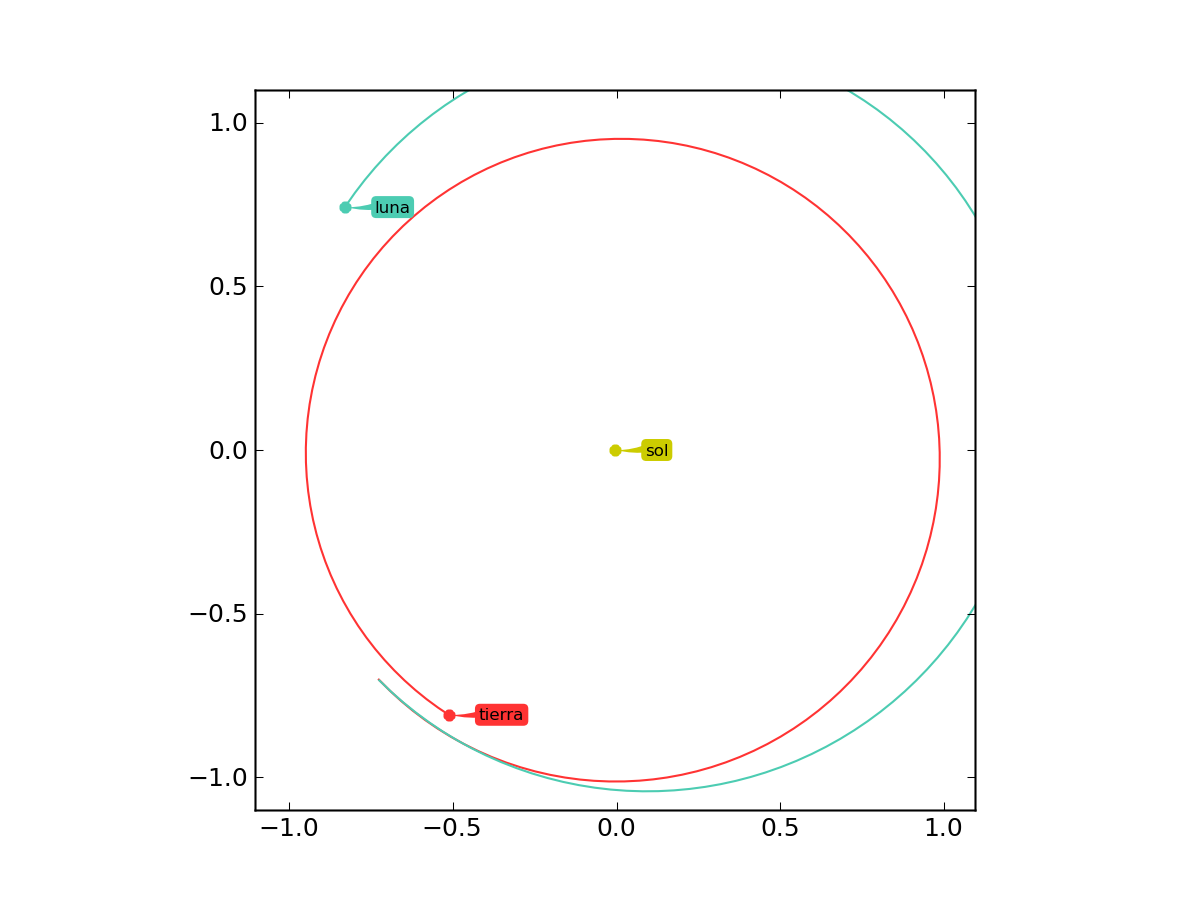
\includegraphics[scale=0.38]{img/ej1/metodo2/validacion_365_4.png}
	\label{fig:ej1_m2_365_4}
	}
	\\
	\subfigure[$\Delta t$ = 2 horas]{
	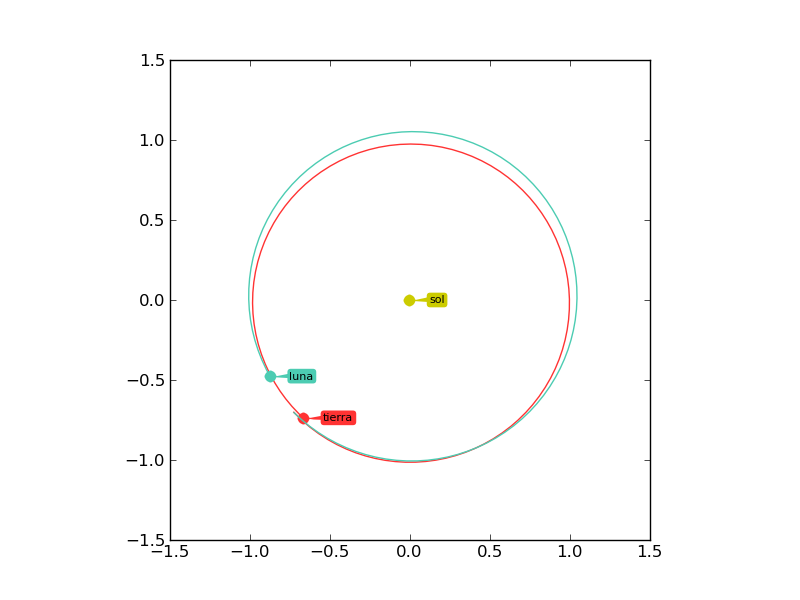
\includegraphics[scale=0.38]{img/ej1/metodo2/validacion_365_12.png}
	\label{fig:ej1_m2_365_12}
	}
	\subfigure[$\Delta t$ = 1 hora]{
	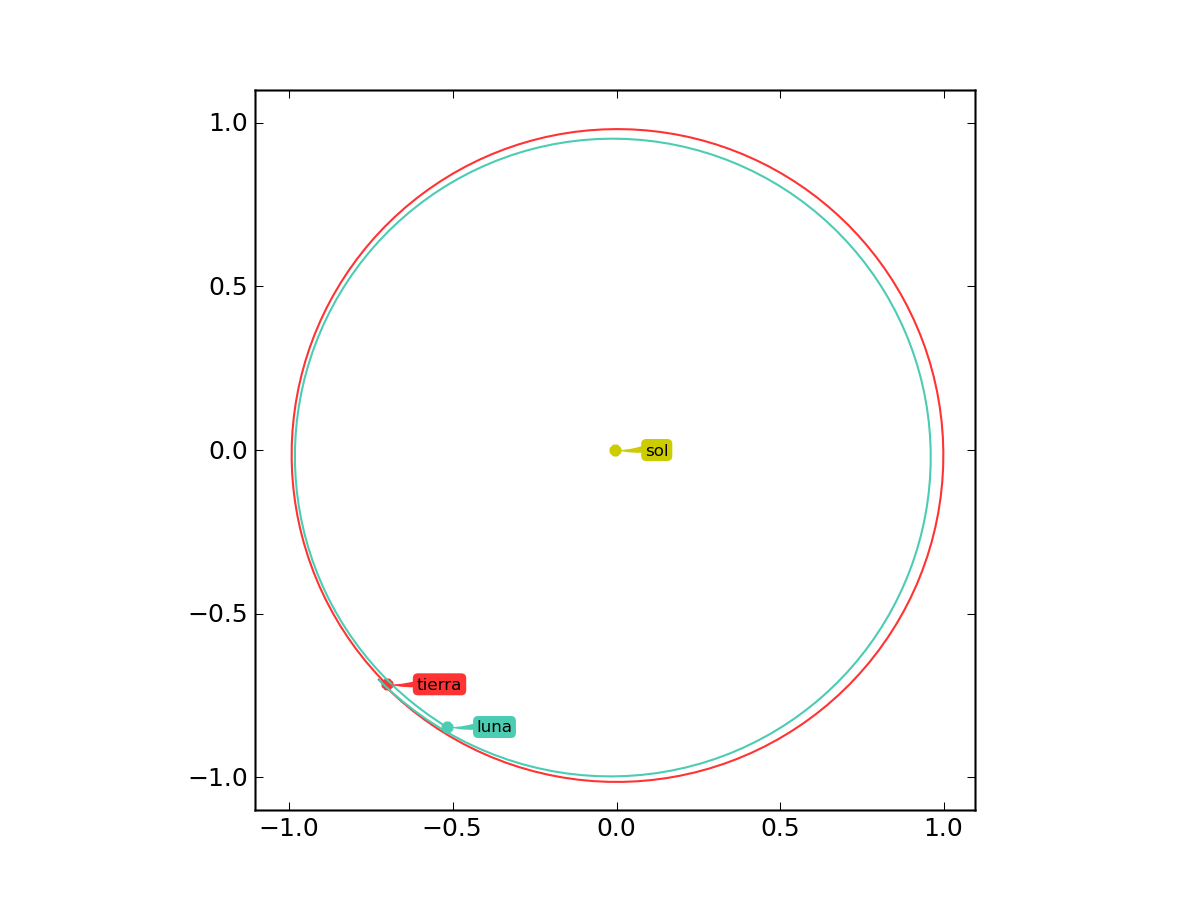
\includegraphics[scale=0.38]{img/ej1/metodo2/validacion_365_24.png}
	\label{fig:ej1_m2_365_24}
	}
	\caption{
		Simulación de validación del sistema sol$-$tierra$-$luna para un período de 1 año y distintos $\Delta t$
		con el método 2.
		Para este método en este tiempo de simulación ya podemos descartar el $\Delta t$ de 6 horas como simulación razonable,
		cuando con el método 1 para este período de tiempo solo descartabamos el $\Delta t$ de 1 día.
		Sigue manifestándose entonces la alta sensibilidad a los errores por discretizacion del tiempo.
	}
	\label{ fig:res_ej1_m2_365 }
\end{figure}
\begin{figure}
	\centering
	\subfigure[$\Delta t$ = 1 día]{
	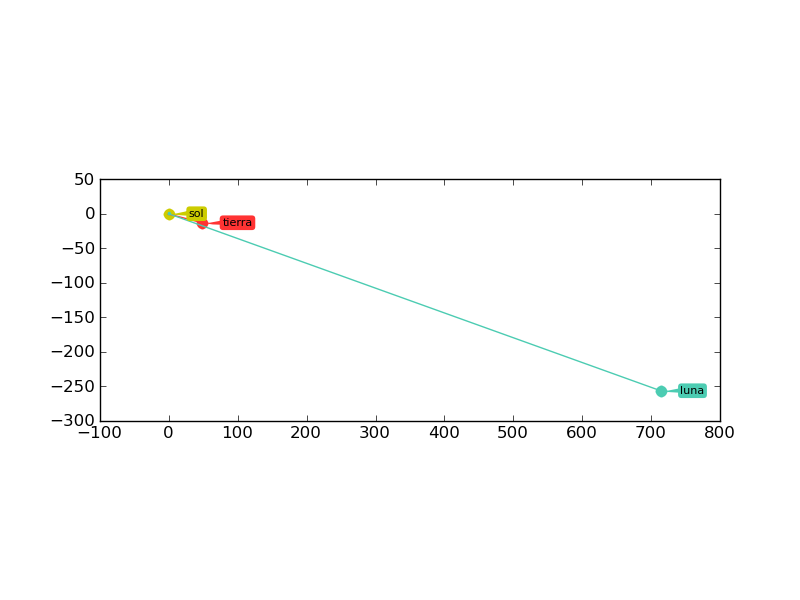
\includegraphics[scale=0.38]{img/ej1/metodo2/validacion_1825_1.png}
	\label{fig:ej1_m2_1825_1}
	}
	\subfigure[$\Delta t$ = 6 horas]{
	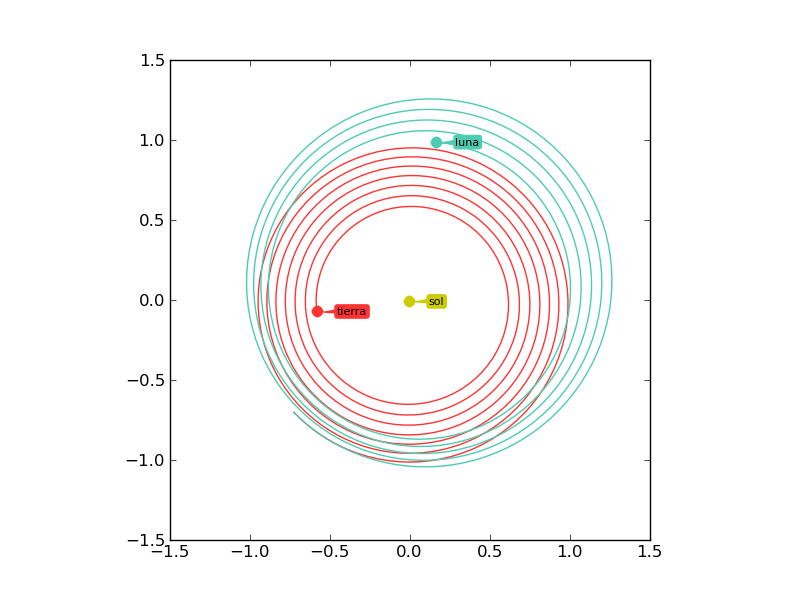
\includegraphics[scale=0.38]{img/ej1/metodo2/validacion_1825_4.png}
	\label{fig:ej1_m2_1825_4}
	}
	\\
	\subfigure[$\Delta t$ = 2 horas]{
	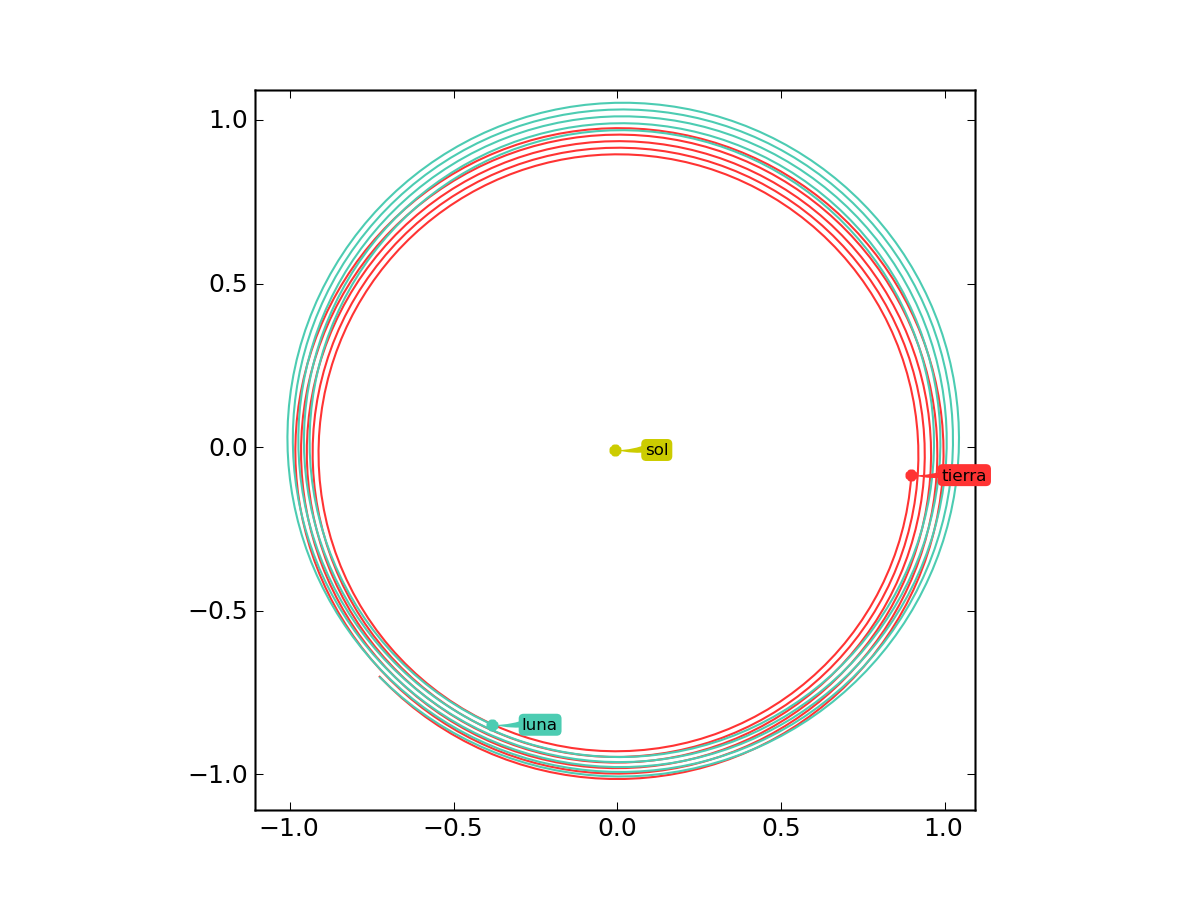
\includegraphics[scale=0.38]{img/ej1/metodo2/validacion_1825_12.png}
	\label{fig:ej1_m2_1825_12}
	}
	\subfigure[$\Delta t$ = 1 hora]{
	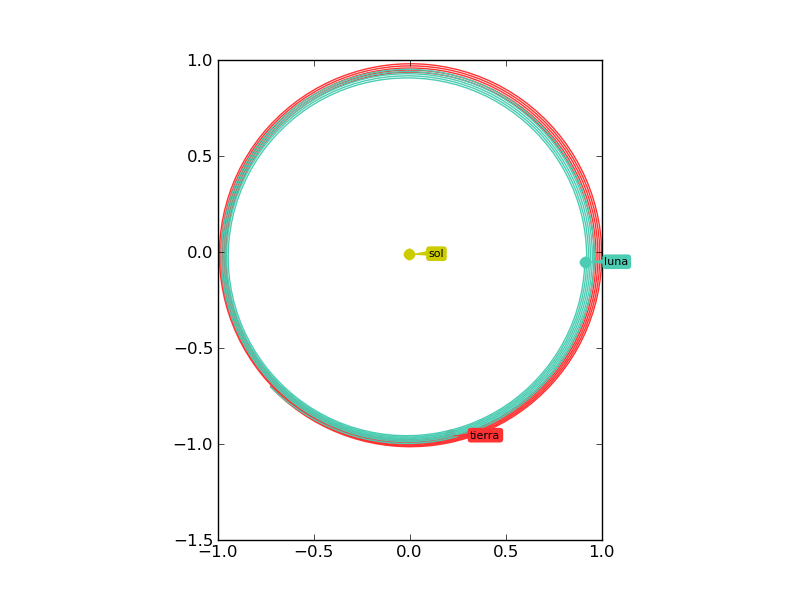
\includegraphics[scale=0.38]{img/ej1/metodo2/validacion_1825_24.png}
	\label{fig:ej1_m2_1825_24}
	}
	\caption{
		Simulación de validación del sistema sol$-$tierra$-$luna para un período de 5 años y distintos $\Delta t$
		con el método 2.
		Acá ya vemos que el único $\Delta t$ razonable que queda es el de 1 hora,
		pero vale la pena notar que es el mejor de los resultados obtenidos hasta ahora en este período de tiempo.
	}
	\label{ fig:res_ej1_m2_1825 }
\end{figure}
